\documentclass[border=1cm]{standalone}
\usepackage{tikz}

\begin{document}
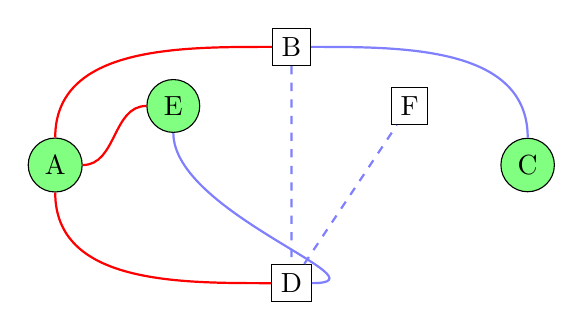
\begin{tikzpicture}[scale=1.5]
    % Define nodes with specified styles
    \node[circle, draw, fill=green!50] at (0,0) (A) {A};
    \node[rectangle, draw, fill=white] at (2,1) (B) {B};
    \node[circle, draw, fill=green!50] at (4,0) (C) {C};
    \node[rectangle, draw, fill=white] at (2,-1) (D) {D};
    \node[circle, draw, fill=green!50] at (1,0.5) (E) {E};
    \node[rectangle, draw, fill=white] at (3,0.5) (F) {F};
    
    % Draw triangle BDF with dashed light blue lines
    \draw[blue!50, dashed, thick] (B) -- (D) -- (F) -- cycle;
    
    % Draw red arcs
    \draw[red, thick] (B) to[out=180, in=90] (A);
    \draw[red, thick] (D) to[out=180, in=270] (A);
    \draw[red, thick] (A) to[out=0, in=180] (E);
    
    % Draw blue arcs
    \draw[blue!50, thick] (B) to[out=0, in=90] (C);
    \draw[blue!50, thick] (D) to[out=0, in=270] (E);
    
\end{tikzpicture}
\end{document}